\documentclass{article}

\usepackage[english]{babel}
\usepackage[letterpaper,top=2cm,bottom=2cm,left=3cm,right=3cm,marginparwidth=1.75cm]{geometry}

\usepackage{amsmath}
\usepackage{graphicx}
\usepackage[colorlinks=true, allcolors=blue]{hyperref}

\title{Homework 1 Solutions}
\author{Microl Chen}

\begin{document}
\maketitle

\section{Collaboration Statement}
For this assignment, the following resources, help, or/and collaboration was utilized:
\\Overleaf - for the Latex Template
\\Stack Overflow - for pandas formulas and syntax


\section{Task 1 Attribute Description}
Semester - Categorical Ordinal - This could be both ordinal or nominal depending on the situation. Although one could argue that the numbers in the semesters are for naming purposes only, the timeline of which semesters came first (ordinance) of the semesters is very important.
\\\\Student ID - Nominal Categorical - a student ID has no significant ordering, and the serial numbers serve simply as a reference id.
\\\\Name - Nominal Categorical - Names don't have order.
\\\\Section -  Nominal Categorical - Although there is numbering on the sections, there is no inherent ranking to be made and the numbers are simply use as references.
\\\\Home Works (1-5) - Numerical Interval - There is no ratio in the scores. 20 points does not necessarily imply that the student did 2 times better than a student who receive 10 points. Similarly, there is no true 0, as a score of 0 could mean that a student got all problems wrong or the assignment was simply not turned in.
\\\\Peer Evaluation - Numerical Interval - Same explanation as home works.
\\\\Bonus - Numerical Ratio - This is another grey area. A student that gets 4 bonus points turned in 2 times more assignments early than a student who received 2 points. The numbers could be direct ratios of each other. Lastly, a true 0 here would represent not turning in any assignments early.
\\\\Quizes (1-12) - Numerical Interval - Same explanation as home works.
\\\\Quiz Adjustments - Numerical Interval - This is a grey area, but the attribute feels like an alternative quiz, so I would apply the same reasoning to that of quizzes.
\\\\Drop Lowest Scores (1-2)  - Numerical Ratios - Although there shouldn't be negative signs with numerical ratios, in this scenario, the negative sign is more or less symbolic. It just tells us we want to subtract a positive amount of points. The scores being drop are also directly proportional to each students total score and a true 0 exist in that it will represent that no scores were dropped.
\\\\Final Exam  - Numerical Interval - Same explanation as home works.
\\\\Total Score  - Numerical Interval - Same explanation as home works.
\\\\Letter Grade - Categorical Ordinal - There is rank between each letter grade.

\section{Task 2 Missing Values}
\subsection{Home works, Peer Evaluation, Quizzes, and Final Exam} 
For these assignment type attributes, missing values most likely means the assignment was not turned in or completed. This would mean that the best value to input for these situations is "0" since not completing an assignment results in 0 points. It would make the data very straight forward. I don't for see any cons here given this reasoning.
\subsection{Bonus}
For bonuses, a missing value would mean no bonuses was completed by the student, so a "0" would also suffice in those areas. Like the previous set of attributes, I also do not see any cons with this decision. 
\subsection{Quiz Adjustments}
This value is a bit more harder since we are not given how these points are utilize to help calculate the students final scores. My best guess is that its a value that is thrown into a formula with the rest of the quiz scores to manipulate the quiz average. Missing values here would mean such manipulation was not necessary. If my speculation was correct, we should not put any values here if they are missing as adding 0 or any other number might skew the average. The cons of doing this is that we may have to change our formulas because we can not simply run a program on an empty variable if it expects an integer. For this reason, we may consider using the median or mean of the students quiz scores to fill this. 

\section{Task 3 Re-encoding}
When we manipulate data, the best practice (especially for people working with machine learning data) is to type set the data into a numerical representation so that we can easily communicate notions of order and rank (or any other properties) into something the computer understands. With the current data set, the semester data are represented with F and S for spring and fall. These letters come first and are sorted alphabetically and this does not reflect the timeline that we want to represent. To fix this, we can either re-encode the data with their year first or completely map each semester into an numerical integer by moving the F and S to end of the number and converting F into a 0 and S into a 1 (S17 would become 171), and sorting this would give us their time line order. For this assignment however, the first method would suffice as we can easily sort it by string comparison with the data set we were given. As for the section data, it is already numeric, and we do not really have to improve upon it.

\section{Task 4 Scaling and z-scoring}
\subsection{Method 1: Intuitive Re-scaling}
This method gives us a good understanding of a student's relative performance compared to the best performing and worst performing scores. The method has major issues if we try to extrapolate any other information. For instance, if one student scored a 100, and every other student scored a 40, it would seem like all the other students performed below the mean. In addition, this method would not be able to differentiate a scenario where all the students scored 50 out of 100 points from one where all the students scored 90 out of 100 since the highest score is mapped onto 100.
\subsection{Method 2: Z-Score Re-scaling}
This method gives us a good understanding of a student's relative performance to their peers (notices how each student is not compared to the best and worst student but that of the average). A z-score shows us whether a student is performing substantially different than everyone else, and it is by far one of the best relative comparison statistic we can look at.
\subsection{Method 3: Group Specific Z-Score Re-scaling}
This method is almost identical to the previous one so the same comments apply. The only difference is that this method would also control for the minute differences between how each semester might be taught.
\\\\Appropriate Method: A good argument could be made for both methods 2 and 3, but since all the data is present, I would assume we would also want to see if there is significant differences in z score across semesters so it would seem like method 2 would be most appropriate. If we pick method 3, we might be able to better track an individual's performance but method 2 allows for a comparison across time. Personally, I also know that the same professor teaches CS170 each semester, so it may not make sense to control for individual semesters.

\section{Task 5 Summary Statistics}
Homework 1 
Mean: 37.785 Std: 7.251 Max: 44.0 Min: 0.0
Q1: 37.0 Median: 40.0 Q3: 42.0
\\Homework 2 Mean: 37.984 Std: 6.332 Max: 44.0 Min: 0.0
Q1: 37.0 Median: 40.0 Q3: 41.0
\\Homework 3 Mean: 37.471 Std: 6.901 Max: 44.0 Min: -7.0
Q1: 36.0 Median: 40.0 Q3: 42.0
\\Homework 4 Mean: 
37.993 Std: 6.747 Max: 44.0 Min: -3.0
Q1:    37.0 Median:    40.0 Q3:    42.0
\\Homework 5 Mean: 40.096 Std: 6.363 Max: 44.0 Min: 0.0
Q1:    40.0 Median    42.0 Q3:    42.0
\\Peer Evaluations Mean: 146.591 Std: 16.185 Max: 150.0 Min: 1.0
Q1:    150.0 Median:    150.0 Q3:    150.0
\\Quiz 01 Mean: 38.649 Std: 11.314 Max: 50.0 Min: 5.0
Q1:    30.0 Median:    43.0 Q3:    49.0
\\Quiz 02 Mean: 42.769 Std: 9.912 Max: 50.0 Min: 0.0
Q1:    39.0 Median:    46.0 Q3:    50.0
\\Quiz 03 Mean: 34.319 Std: 10.799 Max: 50.0 Min: 1.0
Q1:    28.0 Median:    37.0 Q3:    42.0
\\Quiz 04 Mean: 41.818 Std: 8.493 Max: 50.0 Min: 0.0
Q1:    39.0 Median:    45.0 Q3:    48.0
\\Quiz 05 Mean: 36.635 Std: 11.718 Max: 50.0 Min: 0.0
Q1:    30.0 Median:    40.0 Q3:    46.0
\\Quiz 06 Mean: 34.119 Std: 11.679 Max: 50.0 Min: 2.0
Q1:    26.0 Median:    37.0 Q3:    43.0
\\Quiz 07 Mean: 34.383 Std: 13.025 Max: 50.0 Min: 0.0
Q1:    25.0 Median:    37.0 Q3:    46.0
\\Quiz 08 Mean: 32.702 Std: 14.190 Max: 50.0 Min: 0.0
Q1:    23.0 Median:    36.0 Q3:    44.0
\\Quiz 09 Mean: 30.291 Std: 12.335 Max: 50.0 Min: 0.0
Q1:    21.0 Median:    30.0 Q3:    40.0
\\Quiz 10 Mean: 31.056 Std: 11.495 Max: 50.0 Min: 0.0
Q1:    23.0 Median:    32.0 Q3:    41.0
\\Quiz 11 Mean: 37.782 Std: 14.850 Max: 50.0 Min: 0.0
Q1:    31.0 Median:    44.0 Q3:    50.0
\\Quiz 12 Mean: 36.823 Std: 15.340 Max: 50.0 Min: 0.0
Q1:    28.0 Median:    43.0 Q3:    50.0
\\Final Exam Mean: 109.550 Std: 21.071 Max: 147.0 Min: 24.0
Q1:     99.0 Median:    114.0 Q3:    126.0
\\Total Score Mean: 798.955 Std: 185.857 Max: 1000.0 Min: 0.0
Q1:    738.75 Median:    852.50 Q3:    926.00
\\Drop Lowest Quiz 1 Mean: -14.279 Std: 13.615 Max: 0 Min: -48
Q1:   -26.0 Median:   -13.0 Q3:     0.0
\\Drop Lowest Quiz 2 Mean: -21.626 Std: 13.773 Max: 0.0 Min: -49.0
Q1:   -32.25 Median:   -24.00 Q3:   -10.00

\section{Task 6 Charts}
\subsection{Figure 1} 
Figure 1 is a box plot showing the Q1, median, and Q3 points among all the students for each individual homework. From the figure, we can see instances of outliers (those outside the box plot) as well as how skewed the data for each individual homework is. With this data, one could make assumptions on the difficulty of the home works relative to each other. For this figure specifically, we observe that the performance of each home work was more or less similar, so we can imply that the difficult was also similar.

\subsection{Figure 2}
Figure 2 is a box plot showing the Q1, median, and Q3 points among all the students for home work 1 re scaled or normalized with different methods. In retrospect, this figure may not have been the best way to represent the data as the resizing methods inherently produces drastically different values, hence we can not learn much from this figure.

\subsection{Figure 3}
Figure 3 is very similar to figure 1. It is a box plot showing the Q1, median, and Q3 points among all the students for each individual homework normalized to a z-score. Since the data is normalized to z-scores, this figure provides an even more accurate depiction on relative differences in points from each homework. It is interesting to observe that the variability decreases as the semester goes on. At the earlier home works, the IQR had a bigger range, meaning that alot more students were achieving points far from the mean compared to the later homeworks. This implies that as students got use to completing the homeworks, many more students are more consistently performing on a satisfactory level -resulting in a smaller variability and higher mean.

\subsection{Figure 4}
Figure 4 is a histogram that shows the distribution of students' home work 1 and home work 5 scores. The figure shows us an estimate of how students scored 10, 20, 30, or 40 points respectively. From the figure, we can gather that the points are drastically skewed (which is a good thing for grades). Additionally, the figure also shows about 200 more students scored 40 or above in homework 5 compared to homework 1. This finding further supports the idea that the student's performance in terms of scoring well on homeworks increased as they have been exposed to more home works.

\subsection{Figure 5}
Figure 5 is very similar to figure 4, instead of homework 1 and homework 5, this histogram shows the distribution for quiz 1 and quiz 12. In this figure, it is surprising to find a different trend compared to figure 4. Instead of becoming more skewed, we see that the final quiz (12) distribution grows into one more leveled. The counts for the lower scores were the one to increased. I suspect that this is because the quizzes grew harder towards the end of the semester.

\subsection{Figure 6}
Figure 6 compares the distribution of final exam scores and the distribution of total scores. The interesting thing to note from this figure is that the final exam distribution looks more normal while the total score distribution is skewed. The observation to be made here is that students did not needed a perfect score on the final exam to achieve a near perfect score total. This shows us how effective the bonus points and quiz adjustments are.

\subsection{Figure 7}
Figure 7 is a scatter plot comparing total scores and homework 1. This figure shows us if there is a strong correlation between doing well on your home work and obtaining a good total score. From the figure, we see that there is many points at the top right, meaning most students with high home work 1 points also received high total scores, however, what is interesting is that a correlation could not be significantly established. There are enough data points to show that home work 1 did not have a significant weight on the total score.

\subsection{Figure 8}
Figure 8 is more or less the same as figure 7. Instead of looking at homework, this figure examines quiz 1 and maps it onto the total score. Like figure 7, we do not see a significant correlation between these two variables.

\subsection{Figure 9}
Figure 9 is a scatter plot that, like figure 7 and 8, seeks to determine the correlation of two variables - in this case the final exam and total score. Unlike the previous two figures, however, we actually see a strong positive correlation between these two variables. Looking at the trend, we can make a strong case that higher final exam scores equate to higher total scores. We are not surprise to find this finding as the final is one assignment that is worth a large portion of the final grade.

\subsection{Figure 10}
Figure 10 looks to examine the correlation between home work and total score again, but at a different perspective. Previously, we map a single home work (1) onto total scores and we did not find a correlation. In this figure, we seek to find the correlation of the mean of all home works and total scores. Unsurprisingly, we find a positive correlation. We know that home work makes up a large portion of the total score, so doing well on average across your homeworks is necessary to receive that portion. We did not see an indication of any significant correlation in our previous figure (7) because each individual homework is worth considerably less then the aggrgate.

\begin{figure}
\centering
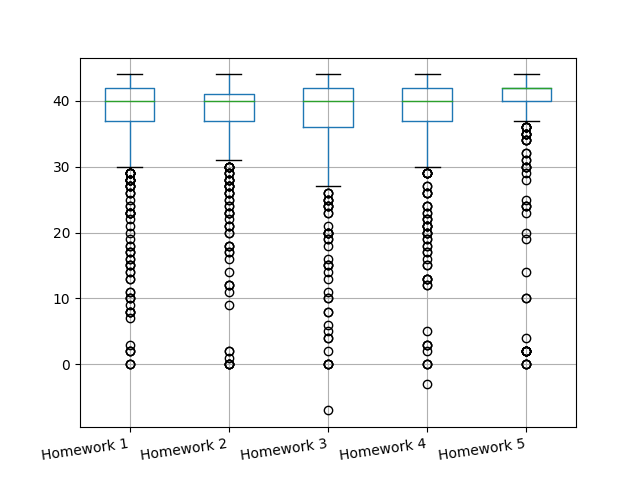
\includegraphics[width=0.3\textwidth]{bx1.png}
\caption{\label{fig:bx1} Box plot of all home work points.}
\end{figure}
\begin{figure}
\centering
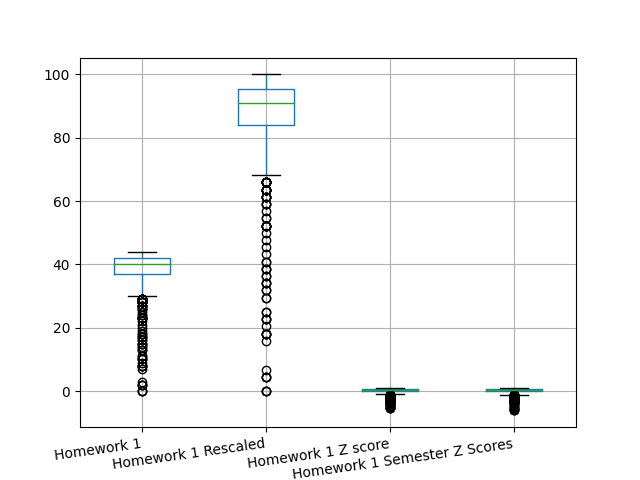
\includegraphics[width=0.3\textwidth]{bx2.png}
\caption{\label{fig:bx2} Box plot comparing the distribution of home work points with different normalization.}
\end{figure}
\begin{figure}
\centering
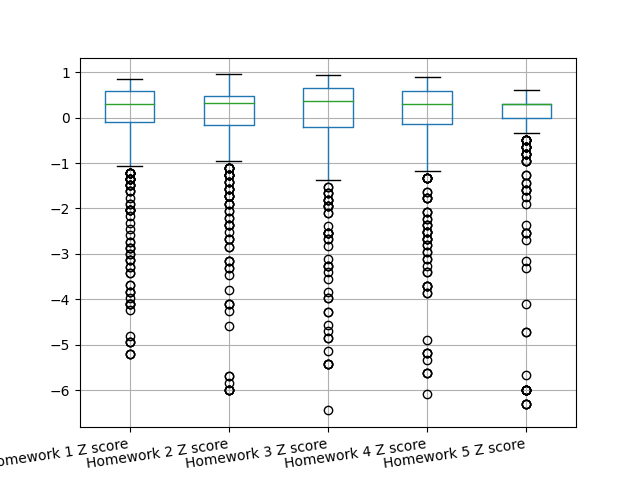
\includegraphics[width=0.3\textwidth]{bx3.png}
\caption{\label{fig:bx3} Box plot of all home work points normalized to z scores.}
\end{figure}
\begin{figure}
\centering
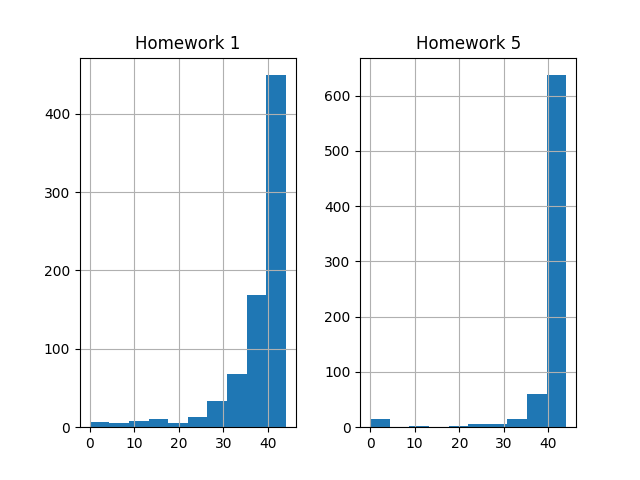
\includegraphics[width=0.3\textwidth]{hx1.png}
\caption{\label{fig:hx1} Histogram of home work 1 and home work 5 respectively.}
\end{figure}
\begin{figure}
\centering
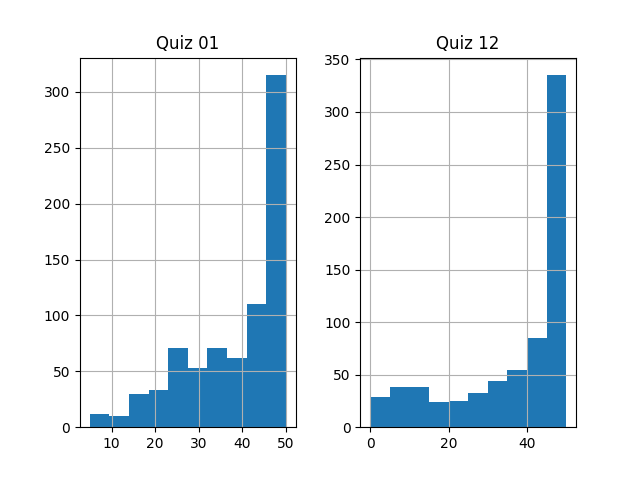
\includegraphics[width=0.3\textwidth]{hx2.png}
\caption{\label{fig:hx2} Histogram of quiz 1 and quiz 12 respectively.}
\end{figure}
\begin{figure}
\centering
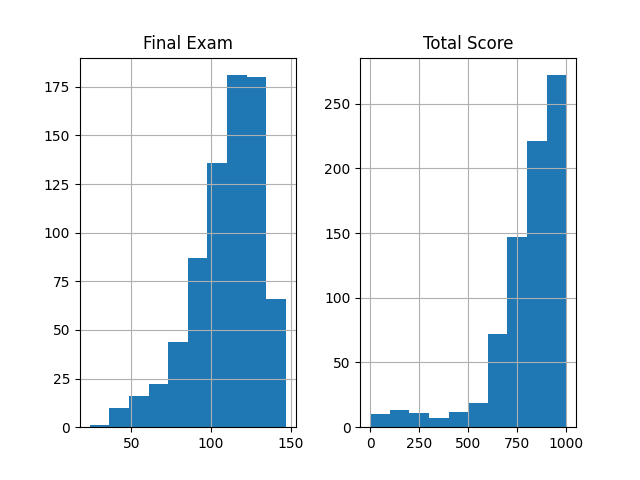
\includegraphics[width=0.3\textwidth]{hx3.png}
\caption{\label{fig:hx3} Histogram of final exam and total score respectively.}
\end{figure}
\begin{figure}
\centering
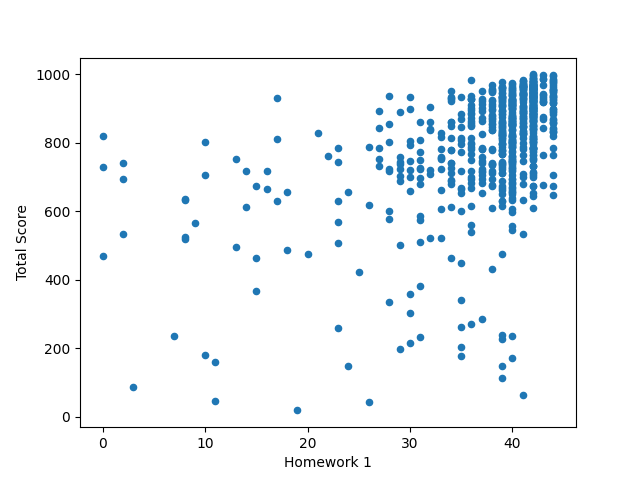
\includegraphics[width=0.3\textwidth]{sx1.png}
\caption{\label{fig:sx1}Scatter plot of total score versus home work 1 points.}
\end{figure}
\begin{figure}
\centering
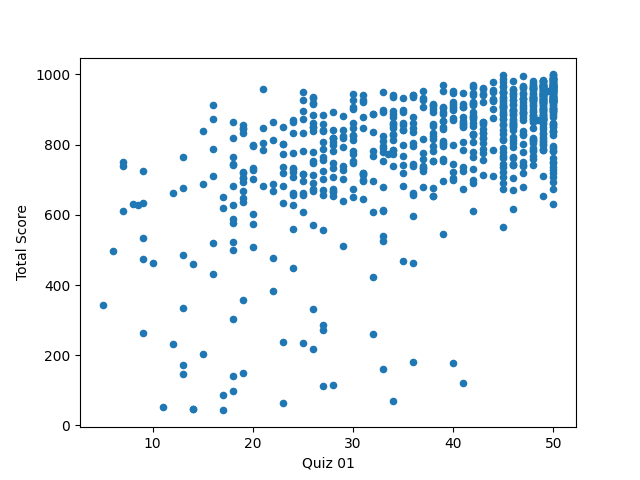
\includegraphics[width=0.3\textwidth]{sx2.png}
\caption{\label{fig:sx2} Scatter plot of total score versus quiz 1 points.}
\end{figure}
\begin{figure}
\centering
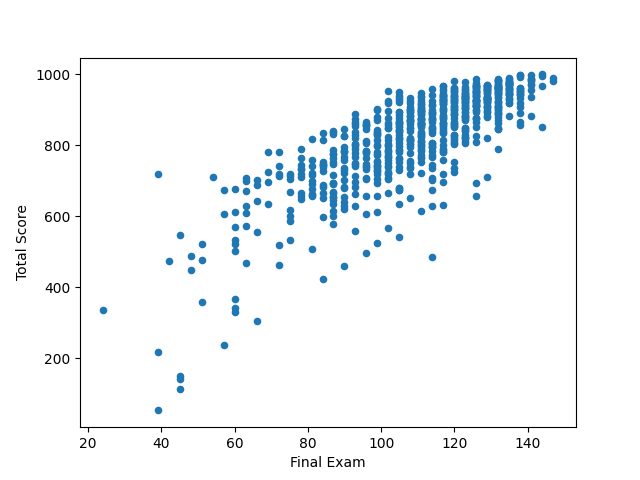
\includegraphics[width=0.3\textwidth]{sx3.png}
\caption{\label{fig:sx3} Scatter plot of total score versus final exam points.}
\end{figure}
\begin{figure}
\centering
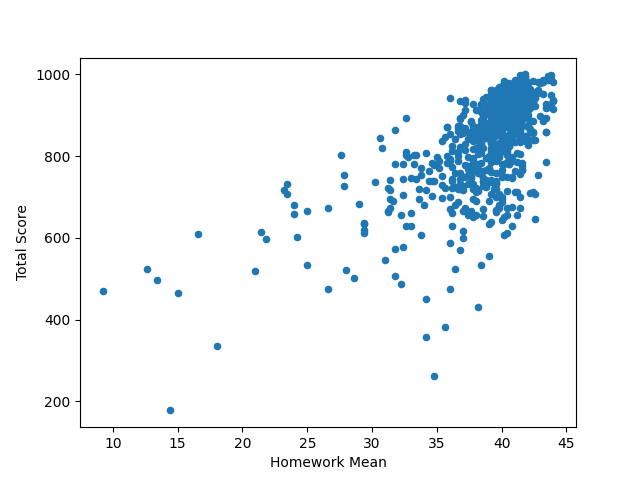
\includegraphics[width=0.3\textwidth]{dx1.png}
\caption{\label{fig:dx1} Scatter plot of total score versus home work means.}
\end{figure}

\section{Task 7 Tools and languages}
For this home work assignment, the primary tools I have chosen to use was Pycharm (python) and Overleaf (latex). I have not have experience with either, but I found that there are so many helpful tutorials online - especially regarding pandas in python. Pandas enable us to access data stored in csv files with rudimentary one-lined commands and it is very intuitive. As for latex, it felt overwhelming at first since this is was my first time using latex, yet the initial template on Overleaf had examples of all the basic things one needed to know. It was a great opportunity to learn simply by editing latex syntax that was already given to us. 

\section{Task 8 Latex document}
Python files for my csv generation as well as all the data cleaning and formulation could be found in a sub folder of the zip file. Dataprocessing.py is the main file with all the cleaning and calculation and test.py is the file that contains the codes for the figure generations.

The latex source code and csv file can be found within the zip file.

The figures are located in a subfolder.
\end{document}